\documentclass[a4paper,12pt]{article}

% Packages
\usepackage[T1]{fontenc}
\usepackage{lmodern}
\usepackage[utf8]{inputenc}
\usepackage{graphicx}  % For images
\usepackage{listings}  % For code snippets
\usepackage{xcolor}    % For code coloring
\usepackage{hyperref}  % For hyperlinks
\usepackage{amsmath}   % For math equations
\usepackage{caption}   % Better captions
\usepackage{geometry}  % Page layout
\usepackage{float}     % For [H] float placement
\geometry{margin=2.5cm}
\usepackage{tikz}
\usepackage{pgfplots}
\pgfplotsset{compat=1.18}
\pgfplotsset{
    colormap={gray}{
        rgb255=(255,255,255)
        rgb255=(0,0,0)
    }
}

% Remove paragraph indentation
\setlength{\parindent}{0pt}

% Code styling
\lstset{
    language=Python,
    basicstyle=\ttfamily\footnotesize,
    keywordstyle=\color{blue},
    stringstyle=\color{red},
    commentstyle=\color{gray},
    breaklines=true,
    frame=single
}

\title{ \textbf{Motion Recognition using IMU Sensor Fusion}}
\author{Sahil Gore \\ 12505425  \\ Embedded Systems \\ Instructor: Prof. Tobias Schaffer}
\date{5 July 2025}

\begin{document}

\maketitle

\section{Introduction}
Gesture recognition using motion sensors offers an intuitive way of interacting with embedded systems. In this lab, we developed a motion recognition system using a Raspberry Pi and Sense HAT, which provides IMU data from an accelerometer and gyroscope.

We collected and labeled the motion data for four gestures and used them to train a simple neural network. The trained model was converted to TensorFlow Lite and deployed on a Raspberry Pi. Based on real-time sensor readings, the system classifies the gesture and displays the result using the LED matrix. This project demonstrates how AI enables control using low-cost hardware.

\section{Objective}
To collect IMU sensor data, classify motion types in real time using a trained neural network, and provide visual feedback via the Sense HAT.

\section{Hardware and Software Used}
\begin{itemize}
    \item \textbf{Hardware:} Raspberry Pi 4 Model B, Sense HAT (IMU: accelerometer + gyroscope)
    \item \textbf{Software:} Raspberry Pi OS, Python 3.9+, TensorFlow, NumPy, TensorFlow Lite, scikit-learn
\end{itemize}

\section{Methodology}
The methodology of this project consists of collecting IMU sensor data, training a neural network model to classify gestures, and deploying the model on a Raspberry Pi for real-time inference. 

\subsection*{GitHub Repository}
\begin{itemize}
    \item \textbf{Code Repository:} \url{https://github.com/LoKI-Codestar/IMU_motion_recognition}
\end{itemize}

\subsection*{Data Collection}
Sensor readings (accelerometer and gyroscope) are recorded at 50 Hz for one second per sample. Data are saved as NumPy arrays in class-labeled folders:

\begin{lstlisting}
import os
import time
import numpy as np
from sense_hat import SenseHat

sense = SenseHat()
LABEL = "move_circle"
SAMPLES = 50
DELAY = 1.0 / 50

save_dir = f"./motion_data/{LABEL}"
os.makedirs(save_dir, exist_ok=True)

input("Press Enter to record 1 second of data")
data = []
for _ in range(SAMPLES):
    acc = sense.get_accelerometer_raw()
    gyro = sense.get_gyroscope_raw()
    sample = [acc['x'], acc['y'], acc['z'], gyro['x'], gyro['y'], gyro['z']]
    data.append(sample)
    time.sleep(DELAY)

np.save(f"{save_dir}/{LABEL}_{int(time.time())}.npy", np.array(data))
\end{lstlisting}

\subsection*{Model Training and Preparation}
The collected data samples are flattened and fed into a fully connected neural network with two hidden layers, trained using TensorFlow. The trained model is converted to TensorFlow Lite format for embedded deployment.

\section{Google Colab Model Training (Code Snippet)}
Below is a snippet of the training code used in Google Colab for building and evaluating the gesture classification model.

\begin{lstlisting}
import numpy as np
import tensorflow as tf
from sklearn.model_selection import train_test_split
from sklearn.preprocessing import LabelEncoder

# Load Data
X = np.load('X_data.npy')
y = np.load('y_labels.npy')

# Preprocess
X = X.reshape((X.shape[0], -1))
le = LabelEncoder()
y_encoded = le.fit_transform(y)

X_train, X_val, y_train, y_val = train_test_split(X, y_encoded, test_size=0.2)

# Model
model = tf.keras.Sequential([
    tf.keras.layers.Dense(128, activation='relu'),
    tf.keras.layers.Dense(64, activation='relu'),
    tf.keras.layers.Dense(len(np.unique(y)), activation='softmax')
])

model.compile(optimizer='adam', loss='sparse_categorical_crossentropy', metrics=['accuracy'])
model.fit(X_train, y_train, validation_data=(X_val, y_val), epochs=20)
model.save('gesture_model.h5')
\end{lstlisting}

\section{Evaluation: Confusion Matrix}
To evaluate the classification accuracy of the model, a confusion matrix was constructed using the validation dataset.

\begin{figure}[h!]
\centering
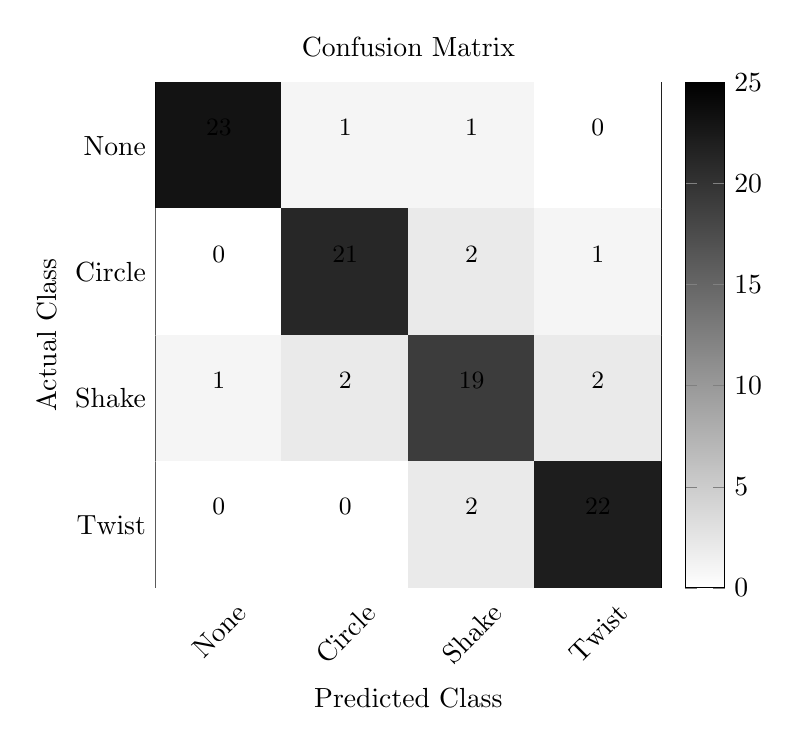
\begin{tikzpicture}
\begin{axis}[
    title={Confusion Matrix},
    xlabel={Predicted Class},
    ylabel={Actual Class},
    xtick=data,
    ytick=data,
    xticklabels={None, Circle, Shake, Twist},
    yticklabels={None, Circle, Shake, Twist},
    enlargelimits=false,
    xticklabel style={rotate=45},
    y dir=reverse,
    colormap name=gray,
    colorbar,
    point meta min=0,
    point meta max=25,
    nodes near coords,
    every node near coord/.append style={font=\small},
    width=8cm,
    height=8cm
]
\addplot[
    matrix plot*,
    mesh/cols=4,
    point meta=explicit
] table [meta=C] {
x y C
0 0 23
1 0 1
2 0 1
3 0 0
0 1 0
1 1 21
2 1 2
3 1 1
0 2 1
1 2 2
2 2 19
3 2 2
0 3 0
1 3 0
2 3 2
3 3 22
};
\end{axis}
\end{tikzpicture}
\caption{Confusion Matrix showing gesture classification results}
\label{fig:confusion_matrix}
\end{figure}

\section{Sensor Output Graphs (6-Axis IMU Signals)}
To better understand how each gesture appears in terms of raw sensor input, we plotted the IMU signals (accelerometer and gyroscope) for each class.

% Include sensor graph images (4 figures with 2 images each)
\begin{figure}[H]
\centering
\includegraphics[width=0.45\linewidth]{move_none_example1.png}
\hfill
\includegraphics[width=0.45\linewidth]{move_none_example2.png}
\caption{Sensor plots for gesture: \texttt{move\_none} (Example 1 and 2)}
\end{figure}

\begin{figure}[H]
\centering
\includegraphics[width=0.45\linewidth]{move_circle_example1.png}
\hfill
\includegraphics[width=0.45\linewidth]{move_circle_example2.png}
\caption{Sensor plots for gesture: \texttt{move\_circle} (Example 1 and 2)}
\end{figure}

\begin{figure}[H]
\centering
\includegraphics[width=0.45\linewidth]{move_shake_example1.png}
\hfill
\includegraphics[width=0.45\linewidth]{move_shake_example2.png}
\caption{Sensor plots for gesture: \texttt{move\_shake} (Example 1 and 2)}
\end{figure}

\begin{figure}[h!]
\centering
\includegraphics[width=0.45\linewidth]{move_twist_example1.png}
\hfill
\includegraphics[width=0.45\linewidth]{move_twist_example2.png}
\caption{Sensor plots for gesture: \texttt{move\_twist} (Example 1 and 2)}
\end{figure}

\section{Real-Time Inference}
On the Raspberry Pi, the TensorFlow Lite model runs inference on incoming 1-second sensor windows. Based on the predicted motion, the Sense HAT’s LED matrix displays a corresponding color.

\begin{lstlisting}
import tensorflow as tf
import numpy as np
from sense_hat import SenseHat
import time

sense = SenseHat()
interpreter = tf.lite.Interpreter(model_path="motion_model.tflite")
interpreter.allocate_tensors()

LABELS = ["move_none", "move_circle", "move_shake", "move_twist"]
COLORS = {
    "move_none": [0, 0, 0],
    "move_circle": [255, 0, 0],
    "move_shake": [0, 255, 0],
    "move_twist": [0, 0, 255]
}

def read_sample():
    acc = sense.get_accelerometer_raw()
    gyro = sense.get_gyroscope_raw()
    return [acc['x'], acc['y'], acc['z'], gyro['x'], gyro['y'], gyro['z']]

while True:
    samples = [read_sample() for _ in range(50)]
    input_data = np.array(samples).flatten().astype(np.float32)
    input_data = np.expand_dims(input_data, axis=0)

    interpreter.set_tensor(interpreter.get_input_details()[0]['index'], input_data)
    interpreter.invoke()
    output = interpreter.get_tensor(interpreter.get_output_details()[0]['index'])[0]

    pred_index = int(np.argmax(output))
    label = LABELS[pred_index]
    sense.clear(COLORS[label])
    time.sleep(0.1)
\end{lstlisting}

\section{Results}
The motion recognition system was tested with four gestures. The model performed low-latency real-time inference and mapped each motion to a unique LED matrix color.

\begin{figure}[htbp]
  \centering
  \begin{minipage}{0.45\textwidth}
    \centering
    \includegraphics[width=\linewidth]{move_none.jpg}
    \caption*{move none}
  \end{minipage}
  \hfill
  \begin{minipage}{0.45\textwidth}
    \centering
    \includegraphics[width=\linewidth]{move_circle.jpg}
    \caption*{move circle}
  \end{minipage}
  \vspace{0.5cm}
  \begin{minipage}{0.45\textwidth}
    \centering
    \includegraphics[width=\linewidth]{move_shake.jpg}
    \caption*{move shake}
  \end{minipage}
  \hfill
  \begin{minipage}{0.45\textwidth}
    \centering
    \includegraphics[width=\linewidth]{move_twist.jpg}
    \caption*{move twist}
  \end{minipage}
  \caption{Real-time results from the Raspberry Pi for each gesture}
  \label{fig:raspberrypi_images}
\end{figure}

\begin{itemize}
    \item \textbf{Accuracy:} Training accuracy ~95\%, validation ~90\%
    \item \textbf{Latency:} ~0.02--0.04 seconds per prediction
    \item \textbf{Color Mapping:}
    \begin{itemize}
        \item move\_none $\rightarrow$ Black
        \item move\_circle $\rightarrow$ Red
        \item move\_shake $\rightarrow$ Green
        \item move\_twist $\rightarrow$ Blue
    \end{itemize}
\end{itemize}

\section{Challenges, Limitations, and Error Analysis}
\begin{itemize}
    \item Sensor noise and gesture overlap led to occasional false predictions.
    \item The dataset was limited in size and diversity.
    \item The system was sensitive to motion execution variations.
\end{itemize}

\section{Discussion}
The project demonstrates real-time AI-based gesture recognition using embedded hardware. Simple models and clean data yielded accurate results. More complex gestures or continuous tracking may require advanced architectures such as CNNs or LSTMs.

\section{Conclusion}
This lab successfully implemented real-time motion recognition using IMU sensor fusion and TensorFlow Lite. The system is effective and low-cost and provides a foundation for future gesture-controlled interfaces.

\section{References}
\begin{itemize}
    \item TensorFlow Lite: \url{https://www.tensorflow.org/lite}
    \item TensorFlow Keras API Guide: \url{https://www.tensorflow.org/guide/keras}
    \item Sense HAT API Documentation: \url{https://pythonhosted.org/sense-hat/}
    \item Goodfellow, Ian, et al. \textit{Deep Learning}. MIT Press, 2016. \url{https://www.deeplearningbook.org/}
    \item Bishop, Christopher M. \textit{Pattern Recognition and Machine Learning}. Springer, 2006.
    \item Scikit-learn documentation: \url{https://scikit-learn.org/stable/documentation.html}
    \item Rajalakshmi, P., \& Anitha, J. (2018). "Gesture Recognition using Accelerometer and Gyroscope Sensors." \textit{International Journal of Engineering \& Technology}, 7(3), 148-151. \url{https://doi.org/10.14419/ijet.v7i3.18.18221}
    \item Raspberry Pi Foundation. "Sense HAT." \url{https://www.raspberrypi.org/products/sense-hat/}
\end{itemize}

\end{document}
